\documentclass{article}

% This document uses the NeurIPS 2024 conference template 
% The NeurIPS template features:
% - Clean, professional typesetting suitable for machine learning publications
% - Two-column layout optimized for conference proceedings
% - Specific formatting for title, authors, sections, and references
% - Support for mathematics and algorithmic content
% - Standardized spacing and margins that follow conference guidelines
%
% Note: The original template has been modified to use Computer Modern Sans Serif
% fonts instead of Helvetica to avoid font compatibility issues.
%
% Load NeurIPS package with "final" option to get camera-ready formatting
\usepackage[final]{neurips_2024}

% Additional packages
\usepackage[utf8]{inputenc} % allow utf-8 input
\usepackage[T1]{fontenc}    % use 8-bit T1 fonts
\usepackage{hyperref}       % hyperlinks
\usepackage{url}            % simple URL typesetting
\usepackage{booktabs}       % professional-quality tables
\usepackage{amsfonts}       % blackboard math symbols
\usepackage{amsmath}        % math equations
\usepackage{amssymb}        % math symbols
\usepackage{float}
\usepackage{mathtools}      % math tools
\usepackage{amsthm}         % theorem environments
\usepackage{nicefrac}       % compact symbols for 1.1, etc.
\usepackage[protrusion=false,expansion=false]{microtype} % microtypography without font expansion
\usepackage{xcolor}         % colors
\usepackage{graphicx}       % figures
\usepackage{subfigure}      % subfigures
\usepackage[capitalize,noabbrev]{cleveref} % better cross-referencing
\usepackage[brazil]{babel}  % brazilian portuguese
\usepackage{array}          % tables
\usepackage{longtable}      % multi-page tables
\usepackage{xcolor}
\definecolor{darkgreen}{rgb}{0.0, 0.5, 0.0}
\title{Avaliação do Modelo BTHOWeN em Datasets Multiclasse}

\author{%
  \begin{tabular}{c@{\hspace{1.5em}}c@{\hspace{1.5em}}c}
    Breno Tostes & Eduardo Naslausky & Felipe Barrocas \\[0.8em]
    Giordano Souza & Maria Bianca Irace & Miguel Sousa \\[0.8em]
    \multicolumn{3}{c}{Rafael Paladini}
  \end{tabular}
  \\[3em]
  COPPE, Universidade Federal do Rio de Janeiro
}

\begin{document}

\maketitle

\begin{abstract}
Este trabalho avalia o modelo BTHOWeN (Bleached Thermometer-encoded Hashed-input Optimized Weightless Neural Network) em diversos datasets multiclasse. Comparamos a performance do BTHOWeN com o modelo BloomWiSARD, analisando o impacto dos hiperparâmetros na acurácia final. Utilizamos uma abordagem gulosa para otimização, variando sequencialmente os parâmetros de tamanho de endereço, número de discriminadores, funções hash, filtros Bloom e fator de bleaching. Os resultados demonstram as vantagens do BTHOWeN em termos de acurácia e eficiência para diversos conjuntos de dados de classificação.
\end{abstract}

\section{Introdução}

A BTHOWeN (Bleached Thermometer-encoded Hashed-input Optimized Weightless Neural Network) é uma arquitetura de rede neural sem peso que se diferencia do modelo WiSARD (Wilkes, Stonham and Aleksander Recognition Device) \cite{lima2020wisardpkg} por:

\begin{itemize}
    \item Incorporar \textbf{counting} Bloom filters para reduzir o tamanho do modelo e permitir bleaching \cite{santiago2020, santiago2019bloomwisard}. Diferentemente dos Bloom filters tradicionais que armazenam apenas bits (0 ou 1), os counting Bloom filters usados no BTHOWeN mantêm contadores que registram quantas vezes um padrão foi encontrado durante o treinamento, permitindo a aplicação de um limiar de bleaching (threshold) para reduzir o efeito do sobreajuste.
    \item Usar função hash da família H3 que não requer operações aritméticas complexas, consistindo apenas de operações XOR entre bits de entrada e máscaras aleatórias, tornando-a ideal para implementações em hardware com baixo consumo de energia \cite{susskind2022, susskind2024phd}.
    \item Codificação com termômetro não-linear baseado na distribuição gaussiana dos dados, que concentra mais níveis de resolução próximos à média dos dados e menos nos extremos, melhorando assim a acurácia do modelo \cite{susskind2022, santiago2020}.
\end{itemize}

\section{Proposta}
\subsection{Metodologia}

Neste trabalho, iremos replicar o BTHOWeN utilizando o BloomWisard como cerne, com os diferentes datasets multiclasse inclusos no artigo original. A proporção entre a massa de treinamento e a massa de teste foi mantida idêntica às respectivas proporções originais, porém os hiperparâmetros foram configurados para verificar o impacto de cada um deles na acurácia final.

Os hiperparâmetros configuráveis são:

\begin{itemize}
    \item Tamanho do endereço (ou tamanho da tupla).
    \item Número de discriminadores.
    \item Número de funções hash.
    \item Número de filtros de bloom.
    \item Fator do bleaching.
\end{itemize}

Os experimentos são feitos alterando um hiperparâmetro de cada vez, de maneira gulosa. Ao atingir um valor máximo variando apenas um hiperparâmetro, este tem seu valor mantido pelo resto do experimento, e o próximo hiperparâmetro passa a ser o variável. Ao realizar este procedimento com todos os hiperparâmetros, identificamos o melhor resultado.

Tomamos o maior valor de acurácia de todos os experimentos e sua configuração de hiperparâmetros como melhor valor obtido e o comparamos com a acurácia obtida no artigo original.

\subsection{Hiperparâmetros}

\subsubsection{Tamanho do Endereço (Tamanho da Tupla)}

O tamanho do endereço, também conhecido como tamanho da tupla, é um parâmetro da WiSARD que determina a quantidade de bits de entrada agrupados para formar endereços nos filtros de Bloom do BTHOWeN \cite{lima2020wisardpkg, santiago2023}. Este parâmetro afeta o número total de filtros necessários (entradas totais divididas pelo tamanho da tupla) e o espaço de endereçamento de cada filtro.

Tuplas menores resultam em mais filtros e melhor generalização, enquanto tuplas maiores reduzem o número de filtros mas podem comprometer a generalização \cite{santiago2020}. Nos experimentos, este parâmetro varia conforme o dataset, desde valores pequenos (2 para Iris) até valores maiores (28 para MNIST).

\subsubsection{Codificação Termômetro Baseada em Distribuição Gaussiana}

O BTHOWeN implementa uma codificação termômetro não-linear baseada na distribuição gaussiana dos valores de cada característica, diferenciando-se da codificação termômetro padrão com limiares uniformemente espaçados \cite{santiago2020}. Nesta abordagem, se cada característica é codificada com \textit{t} bits, seu intervalo de valores é dividido em \textit{t}+1 intervalos com densidade de probabilidade igual sob uma distribuição normal ajustada aos dados de treinamento \cite{susskind2022}.

Esta técnica posiciona limiares mais próximos entre si perto da média dos dados (maior densidade) e mais espaçados nas caudas da distribuição, alocando maior resolução onde os dados são mais comuns \cite{santiago2020}. Isso otimiza a precisão nas faixas de valores mais frequentes, evitando o desperdício de bits em outliers raros que ocorre com limiares uniformes, o que resulta em melhor performance de classificação.

\subsubsection{Número de Bits por Filtro (OWeN)}

O parâmetro OWeN (Optimized Weightless Neural Network) define o número de bits de entrada mapeados para cada filtro de Bloom dentro de um discriminador \cite{santiago2020}, determinando como o vetor de entrada é particionado entre os filtros. Por exemplo, em um modelo MNIST com entrada de 784 dimensões e OWeN = 28, cada discriminador conteria 28 filtros de Bloom, cada um processando 28 bits específicos da entrada.

A escolha do valor OWeN envolve um trade-off importante \cite{santiago2020, susskind2022}: valores mais baixos resultam em mais filtros com "campos receptivos" menores, potencialmente melhorando a generalização mas aumentando a quantidade de filtros necessários; valores mais altos significam menos filtros com "campos receptivos" maiores, reduzindo a complexidade do modelo mas aumentando o risco de colisões. Nos experimentos do BTHOWeN, os valores de OWeN foram sistematicamente testados para cada dataset (por exemplo, 28, 49 e 56 bits por filtro para MNIST) \cite{santiago2020}.

\subsubsection{Número de Funções Hash (FH)}

O parâmetro FH determina quantas diferentes funções hash são utilizadas em cada filtro de Bloom para mapear os dados de entrada em posições de memória \cite{santiago2020}. O BTHOWeN implementa a família de funções hash H3, que consiste apenas em operações XOR entre bits de entrada e máscaras aleatórias, tornando-a ideal para implementações em hardware \cite{susskind2022}. Uma característica importante é que o BTHOWeN compartilha os mesmos parâmetros aleatórios de hash entre todos os filtros para economizar memória, sem degradar a acurácia \cite{santiago2020}.

O número de funções hash tem uma relação complexa com a taxa de falsos positivos: valores maiores reduzem falsos positivos (todas as k posições precisam colidir para causar um falso positivo), mas aumentam o custo computacional e o número de posições a serem definidas por padrão \cite{santiago2020}. Valores típicos variam de 1 a 6 dependendo do dataset, com o valor ótimo sendo determinado empiricamente para cada caso.

\subsubsection{Número de Filtros de Bloom (FE - Filter Entries)}

O parâmetro FE define o número de entradas em cada filtro de Bloom, ou seja, o tamanho do vetor utilizado para armazenar os padrões aprendidos \cite{santiago2020}. Este tamanho é sempre uma potência de 2 (128, 256, 512, 1024, 2048, etc.).

Aumentar o tamanho do filtro reduz a probabilidade de colisões e a taxa de falsos positivos, mas aumenta a memória necessária \cite{santiago2020, susskind2022}. Este parâmetro afeta diretamente o equilíbrio entre precisão e eficiência de memória do modelo e, em implementações de hardware, traduz-se na quantidade de memória alocada para cada filtro, influenciando diretamente o consumo de energia \cite{susskind2022}.

\subsubsection{Limiar de Bleaching (b)}

O limiar de bleaching é um hiperparâmetro exclusivo da arquitetura BTHOWeN \cite{santiago2020}. Enquanto filtros de Bloom tradicionais armazenam apenas bits (0 ou 1), no BTHOWeN cada posição mantém um contador durante o treinamento, registrando a frequência de cada padrão \cite{santiago2020, lusquino2020}. O parâmetro b define o valor mínimo que um contador deve ter para que um padrão seja considerado válido durante a inferência, funcionando como mecanismo de regularização que filtra padrões pouco frequentes, evitando sobreajuste \cite{carvalho2013bleaching}.

Após o treinamento, um valor ótimo de b é determinado usando um conjunto de validação, geralmente via busca binária \cite{santiago2020, susskind2022}. Os contadores são então binarizados: posições com contadores $\geq$ b se tornam 1, e as demais 0. Na inferência, o modelo considera apenas padrões vistos pelo menos b vezes durante o treinamento. Este processo permite distinguir padrões relevantes de ocorrências aleatórias, melhorando a generalização e beneficiando datasets desbalanceados, onde classes majoritárias poderiam saturar a memória sem este mecanismo \cite{santiago2020}. Valores típicos de b variam de 1 a 20, sendo específicos para cada dataset e configuração.

\subsection{Escolha dos Hiperparâmetros}

A seleção de hiperparâmetros para o BTHOWeN segue uma abordagem iterativa que explora sistematicamente o espaço de configurações. Partindo de baselines para cada dataset, o processo altera um hiperparâmetro por vez, testando múltiplas variações: cinco para bits\_per\_input, seis para filter\_inputs, cinco para filter\_entries e quatro para filter\_hashes. Seguimos uma estratégia gulosa, fixando o melhor valor de cada parâmetro antes de passar ao próximo, o que oferece eficiência computacional e facilita a análise do impacto individual de cada hiperparâmetro.

Para mitigar o risco de convergência para ótimos locais, repetimos o processo com múltiplos pontos de partida e validamos as configurações resultantes com validação cruzada 5-fold. A configuração final é selecionada com base no equilíbrio entre acurácia e robustez, seguida pela determinação do valor ideal de bleaching (testando valores de 1 a 20). Esta metodologia, embora computacionalmente intensiva, garante uma exploração abrangente do espaço de hiperparâmetros e produz configurações que equilibram eficazmente acurácia, eficiência de memória e estabilidade.

% \subsection{Processo de Treinamento e Inferência do BTHOWeN}
%
% O BTHOWeN, como outras redes neurais sem peso baseadas em WiSARD, utiliza um processo de treinamento e inferência significativamente diferente das redes neurais tradicionais baseadas em gradiente. A seguir, descrevemos em detalhes como esses processos funcionam.
%
% \subsubsection{Treinamento (Aprendizado de Passagem Única)}
%
% Uma característica fundamental das redes neurais sem peso é o treinamento de passagem única (one-shot learning), onde cada amostra é apresentada apenas uma vez à rede \cite{santiago2020}. Este processo é determinístico e significativamente mais rápido que o treinamento iterativo de redes neurais convencionais. O processo de treinamento do BTHOWeN segue as seguintes etapas:
%
% \begin{enumerate}
%     \item \textbf{Inicialização:} Todos os contadores nos filtros de Bloom são inicializados com zero.
%
%     \item \textbf{Codificação de Entrada:} Para cada amostra de treinamento, as características são codificadas usando o esquema de termômetro baseado em distribuição gaussiana, gerando um vetor binário.
%
%     \item \textbf{Hashing e Atualização de Memória:} 
%     \begin{itemize}
%         \item O rótulo da amostra determina qual discriminador (classe) aprenderá com essa amostra.
%         \item O vetor binário é dividido em segmentos conforme o parâmetro OWeN e cada segmento é mapeado para um filtro de Bloom.
%         \item Em cada filtro do discriminador da classe correta, as k funções hash H3 são aplicadas ao segmento correspondente para gerar k endereços.
%         \item Os contadores nessas k posições são incrementados em 1.
%     \end{itemize}
%
%     \item \textbf{Seleção do Limiar de Bleaching:} Após processar todas as amostras de treinamento, um conjunto de validação é usado para determinar o valor ótimo do limiar de bleaching b. 
%     \begin{itemize}
%         \item Diferentes valores de b são testados, geralmente usando busca binária.
%         \item O valor que maximiza a acurácia no conjunto de validação é escolhido.
%     \end{itemize}
%
%     \item \textbf{Binarização:} Com o valor b determinado, os contadores são convertidos em bits:
%     \begin{itemize}
%         \item Contadores $\geq$ b são definidos como 1 (padrão memorizado).
%         \item Contadores < b são definidos como 0 (padrão ignorado).
%     \end{itemize}
% \end{enumerate}
%
% Este processo resulta em um modelo binário compacto, onde cada filtro de Bloom contém apenas bits que indicam a presença de padrões vistos pelo menos b vezes durante o treinamento.
%
% \subsubsection{Inferência}
%
% Na fase de inferência, o BTHOWeN segue um processo similar à codificação e hashing da entrada, mas ao invés de atualizar contadores, ele verifica quais padrões armazenados são reconhecidos:
%
% \begin{enumerate}
%     \item \textbf{Codificação:} A amostra de teste passa pela mesma codificação termômetro baseada em distribuição gaussiana.
%
%     \item \textbf{Hashing:} O vetor binário é segmentado e as mesmas funções hash são aplicadas para gerar endereços em cada filtro de Bloom.
%
%     \item \textbf{Verificação de Correspondência:} Para cada discriminador (classe):
%     \begin{itemize}
%         \item Cada filtro de Bloom verifica se todos os k bits nas posições hashadas são 1.
%         \item Se todas as k posições contêm 1, o filtro responde com 1 (padrão reconhecido).
%         \item Se qualquer posição contém 0, o filtro responde com 0 (padrão não reconhecido).
%     \end{itemize}
%
%     \item \textbf{Contagem (Popcount) e Decisão:} 
%     \begin{itemize}
%         \item Para cada discriminador, conta-se quantos filtros responderam com 1, gerando uma pontuação total.
%         \item A classe com a maior pontuação (maior número de filtros ativados) é escolhida como a previsão.
%     \end{itemize}
% \end{enumerate}
%
% É importante notar que o BTHOWeN não utiliza bleaching dinâmico durante a inferência. O limiar de bleaching é fixo e já foi aplicado durante a binarização pós-treinamento, portanto o modelo de inferência trabalha apenas com memória binária e não com contadores.
%
\subsection{Datasets}

\subsubsection{MNIST}

O dataset \textbf{MNIST} (Modified National Institute of Standards and Technology) é uma coleção de dígitos manuscritos. Ele inclui \textbf{60k imagens de treinamento} e \textbf{10k imagens de teste}. Todas as imagens estão em escala de cinza e possuem tamanho de \textbf{28×28 pixels}.

\subsubsection{Ecoli}

O dataset \textbf{Ecoli} é usado para prever onde proteínas celulares se localizam com base em suas sequências de aminoácidos. Ele contém \textbf{336 proteínas}, cada uma descrita por \textbf{sete atributos numéricos} derivados da sequência. As proteínas são classificadas em \textbf{oito possíveis locais celulares}.

\subsubsection{Iris}

O dataset \textbf{Iris} contém \textbf{150 observações} de flores de íris, cada uma descrita por:

\begin{itemize}
    \item Comprimento da sépala.
    \item Largura da sépala.
    \item Comprimento da pétala.
    \item Largura da pétala.
\end{itemize}

A classificação é feita em uma de \textbf{três espécies}: \textbf{Iris Setosa}, \textbf{Versicolor} ou \textbf{Virginica}.

\subsubsection{Glass}

O dataset \textbf{Glass} contém \textbf{214 instâncias} de fragmentos de vidro, cada uma descrita por \textbf{10 atributos}. Com ele, conseguimos prever o tipo de vidro com base em sua composição química e índice de refração.

\subsubsection{Letter}

O dataset \textbf{Letter} contém letras manuscritas. As imagens dos caracteres foram baseadas em \textbf{20 fontes diferentes}, e cada letra dentro dessas fontes foi distorcida aleatoriamente para produzir \textbf{20k entradas}, onde \textbf{16k} foram usadas para treinamento e \textbf{4k} para teste.

\subsubsection{Wine}

O dataset \textbf{Wine} reúne \textbf{178 amostras} de vinho de três cultivares de uvas da região de Piemonte, Itália. Cada amostra é descrita por \textbf{13 atributos químicos contínuos} – como teor de álcool, magnésio e intensidade de cor. O objetivo é identificar a cultivar correta entre as \textbf{três classes} disponíveis.

\subsubsection{Segment}

O dataset \textbf{Image Segmentation} (Segment) contém \textbf{2.310 segmentos} de imagens externas, distribuídos igualmente entre \textbf{sete classes} de região: tijolo, céu, folhagem, cimento, janela, caminho e grama. Cada segmento é representado por \textbf{19 atributos numéricos} que descrevem características de cor e textura. A tarefa é prever a classe da região na qual o segmento se enquadra.

\subsubsection{Shuttle}

O dataset \textbf{Statlog Shuttle} possui cerca de \textbf{58.000 registros} de telemetria do sistema de controle do ônibus espacial. Cada registro é descrito por \textbf{nove atributos numéricos} derivados de sensores a bordo e está rotulado em um de \textbf{sete possíveis estados operacionais}. O conjunto é fortemente desbalanceado, com predominância da classe 1.

\subsubsection{Vehicle}

O dataset \textbf{Vehicle Silhouettes} contém \textbf{846 silhuetas} de veículos, cada uma descrita por \textbf{18 medidas geométricas} extraídas da imagem, como área, compacidade e momentos. Os veículos devem ser classificados em uma de \textbf{quatro categorias}: ônibus, Opel, Saab ou van.

\subsubsection{Vowel}

O dataset \textbf{Vowel Recognition} inclui \textbf{990 amostras} de fala gravadas por 15 locutores. Cada amostra é caracterizada por \textbf{10 atributos acústicos contínuos} (coeficientes derivados do espectro) e deve ser classificada em uma de \textbf{11 vogais} do inglês, como /a/, /e/ ou /i/.

\section{Resultados}

\subsection{Resultados por dataset}

Nas tabelas a seguir, apresentamos os resultados obtidos com diferentes configurações do BTHOWeN para cada dataset. As configurações são organizadas da seguinte forma:

\begin{itemize}
    \item \textbf{Bloom WiSARD}: Resultados obtidos pela implementação original do Bloom WiSARD, apresentados como referência para comparação.
    \item \textbf{Base}: Configuração inicial do BTHOWeN utilizada como ponto de partida para os experimentos, com parâmetros utilizados nos experimentos originais publicados pelo autor.
    \item \textbf{Var. X}: Variações da configuração base, onde modificamos sistematicamente um hiperparâmetro por vez, seguindo a abordagem gulosa descrita na metodologia. Os números indicam a sequência das variações testadas.
\end{itemize}

Para cada configuração, apresentamos os valores dos hiperparâmetros (b, OWeN, FE, FH), a acurácia obtida, o percentual de empates ocorridos durante a classificação e o valor de bleaching que produziu os melhores resultados. A coluna ``Bleaching'' indica o valor ótimo encontrado durante o treinamento, que permite ao modelo obter a melhor acurácia possível.

\subsubsection{Tabelas}

{\small
\begin{table}[H]
\caption{Parâmetros e métricas do dataset Iris}
\begin{tabular}{|c|c|c|c|c|c|c|c|}
\hline
\textbf{Configuração} & \textbf{b} & \textbf{OWeN} & \textbf{FE} & \textbf{FH} & \textbf{Acurácia} & \textbf{Empates (\%)} & \textbf{Bleaching} \\
\hline
Bloom WiSARD & N/A & N/A & N/A & N/A & 960 & 2.0 & 3 \\
\hline
Base & 3 & 2 & 128 & 1 & 980 & 12.0 & 2 \\
\hline
Var. 1 & 4 & 2 & 128 & 1 & 920 & 16.0 & 1 \\
\hline
Var. 2 & 3 & 2 & 256 & 1 & 980 & 14.0 & 2 \\
\hline
Var. 3 & 3 & 2 & 128 & 2 & 980 & 8.0 & 2 \\
\hline
Var. 4 & 4 & 2 & 128 & 2 & 860 & 4.0 & 9 \\
\hline
\textbf{Var. 5} & 3 & 2 & 256 & 2 & \textbf{980} & \textbf{0.0} & 2 \\
\hline
Var. 6 & 4 & 2 & 256 & 2 & 900 & 12.0 & 3 \\
\hline
\end{tabular}
\end{table}

\begin{table}[H]
\caption{Parâmetros e métricas do dataset Ecoli}
\begin{tabular}{|c|c|c|c|c|c|c|c|}
\hline
\textbf{Configuração} & \textbf{b} & \textbf{OWeN} & \textbf{FE} & \textbf{FH} & \textbf{Acurácia} & \textbf{Empates (\%)} & \textbf{Bleaching} \\
\hline
Bloom WiSARD & N/A & N/A & N/A & N/A & 799 & N/A & N/A \\
\hline
Base & 10 & 128 & 2 & 10 & 786 & 8.9 & 7 \\
\hline
Var. 1 & 4 & 128 & 2 & 11 & 821 & 10.7 & 1 \\
\hline
Var. 2 & 3 & 256 & 2 & 10 & 813 & 19.6 & 1 \\
\hline
Var. 3 & 3 & 128 & 3 & 10 & 786 & 15.2 & 7 \\
\hline
Var. 4 & 4 & 128 & 3 & 11 & 839 & 17.9 & 1 \\
\hline
Var. 5 & 3 & 256 & 3 & 10 & 848 & 10.7 & 1 \\
\hline
Var. 6 & 4 & 256 & 4 & 10 & 830 & 13.4 & 1 \\
\hline
\end{tabular}
\end{table}

\begin{table}[H]
\caption{Parâmetros e métricas do dataset Glass}
\begin{tabular}{|c|c|c|c|c|c|c|c|}
\hline
\textbf{Configuração} & \textbf{b} & \textbf{OWeN} & \textbf{FE} & \textbf{FH} & \textbf{Acurácia} & \textbf{Empates (\%)} & \textbf{Bleaching} \\
\hline
Bloom WiSARD & N/A & N/A & N/A & N/A & 726 & N/A & N/A \\
\hline
Base & 3 & 128 & 3 & 9 & 577 & 39.4 & 1 \\
\hline
Var. 1 & 4 & 128 & 3 & 10 & 563 & 38.0 & 1 \\
\hline
Var. 2 & 3 & 256 & 3 & 9 & 493 & 33.8 & 1 \\
\hline
Var. 3 & 3 & 128 & 4 & 9 & 549 & 19.7 & 4 \\
\hline
Var. 4 & 4 & 128 & 4 & 10 & 592 & 40.8 & 1 \\
\hline
Var. 5 & 3 & 256 & 4 & 9 & 676 & 29.6 & 1 \\
\hline
Var. 6 & 4 & 256 & 4 & 10 & 676 & 28.2 & 1 \\
\hline
\end{tabular}
\end{table}

\begin{table}[H]
\caption{Parâmetros e métricas do dataset Letter}
\begin{tabular}{|c|c|c|c|c|c|c|c|}
\hline
\textbf{Configuração} & \textbf{b} & \textbf{OWeN} & \textbf{FE} & \textbf{FH} & \textbf{Acurácia} & \textbf{Empates (\%)} & \textbf{Bleaching} \\
\hline
Bloom WiSARD & N/A & N/A & N/A & N/A & 848 & N/A & N/A \\
\hline
Base & 3 & 128 & 3 & 9 & 734 & 18.6 & 6 \\
\hline
Var. 1 & 4 & 128 & 3 & 10 & 736 & 17.4 & 5 \\
\hline
Var. 2 & 3 & 256 & 3 & 9 & 789 & 15.2 & 3 \\
\hline
Var. 3 & 3 & 128 & 4 & 9 & 707 & 19.2 & 5 \\
\hline
Var. 4 & 4 & 128 & 4 & 10 & 719 & 18.7 & 6 \\
\hline
Var. 5 & 3 & 256 & 4 & 9 & 775 & 15.6 & 4 \\
\hline
Var. 6 & 4 & 256 & 5 & 12 & 811 & 11.3 & 4 \\
\hline
Var. 7 & 11 & 256 & 5 & 18 & 840 & 7.6 & 3 \\
\hline
Var. 8 & 15 & 256 & 5 & 35 & 884 & 3.9 & 3 \\
\hline
\end{tabular}
\end{table}

\begin{table}[H]
\caption{Parâmetros e métricas do dataset Wine}
\begin{tabular}{|c|c|c|c|c|c|c|c|}
\hline
\textbf{Configuração} & \textbf{b} & \textbf{OWeN} & \textbf{FE} & \textbf{FH} & \textbf{Acurácia} & \textbf{Empates (\%)} & \textbf{Bleaching} \\
\hline
Bloom WiSARD & N/A & N/A & N/A & N/A & 926 & N/A & N/A \\
\hline
Base & 9 & 13 & 128 & 3 & 983 & N/A & 1 \\
\hline
Var. 1.1 & 10 & 13 & 256 & 4 & 1.000 & 1.7 & 1 \\
\hline
Var. 1.1 & 10 & 13 & 256 & 4 & 949 & 3.39 & 1 \\
\hline
Var. 2 & 11 & 9 & 256 & 4 & 983 & 1.69 & 1 \\
\hline
Var. 3 & 11 & 13 & 256 & 2 & 966 & 3.38 & 1 \\
\hline
Var. 4 & 9 & 9 & 256 & 4 & 966 & 1.69 & 1 \\
\hline
Var. 5 & 10 & 17 & 256 & 4 & 966 & 11.8 & 1 \\
\hline
Var. 6 & 11 & 15 & 256 & 2 & 966 & N/A & N/A \\
\hline
Var. 7 & 7 & 9 & 256 & 4 & 932 & 5.08 & 1 \\
\hline
\end{tabular}
\end{table}

\begin{table}[H]
\caption{Parâmetros e métricas do dataset Segment}
\begin{tabular}{|c|c|c|c|c|c|c|c|}
\hline
\textbf{Configuração} & \textbf{b} & \textbf{OWeN} & \textbf{FE} & \textbf{FH} & \textbf{Acurácia} & \textbf{Empates (\%)} & \textbf{Bleaching} \\
\hline
Bloom WiSARD & N/A & N/A & N/A & N/A & N/A & N/A & N/A \\
\hline
Base & 9 & 27 & 1.14 & 2 & 925 & N/A & 1 \\
\hline
Var. 1 & 10 & 16 & 256 & 4 & 938 & 9.35 & 1 \\
\hline
Var. 2 & 8 & 20 & 512 & 3 & 924 & 9.24 & 1 \\
\hline
Var. 3.1 & 10 & 18 & 1.14 & 3 & 942 & 8.57 & 2 \\
\hline
Var. 3.2 & 10 & 18 & 1.14 & 3 & 944 & 6.49 & 2 \\
\hline
Var. 4 & 10 & 20 & 512 & 2 & 944 & 8.96 & 1 \\
\hline
Var. 5 & 16 & 16 & 256 & 3 & 941 & 10.8 & 8 \\
\hline
Var. 6 & 10 & 14 & 512 & 4 & 939 & 8.10 & 2 \\
\hline
Var. 7 & 9 & 20 & 1.14 & 2 & 937 & 23.7 & 1 \\
\hline
Var. 8 & 15 & 15 & 256 & 4 & 936 & 9.8 & 1 \\
\hline
Var. 9 & 9 & 32 & 2048 & 4 & 936 & 34.9 & 1 \\
\hline
\end{tabular}
\end{table}

\begin{table}[H]
\caption{Parâmetros e métricas do dataset Shuttle}
\begin{tabular}{|c|c|c|c|c|c|c|c|}
\hline
\textbf{Configuração} & \textbf{b} & \textbf{OWeN} & \textbf{FE} & \textbf{FH} & \textbf{Acurácia} & \textbf{Empates (\%)} & \textbf{Bleaching} \\
\hline
Bloom WiSARD & N/A & N/A & N/A & N/A & 868 & N/A & N/A \\
\hline
Base & 9 & 27 & 1024 & 2 & 0 & 0 & 0 \\
\hline
Var. 1.1 & 11 & 29 & 1024 & 2 & 999 & 0.11 & 1 \\
\hline
Var. 1.1 & 11 & 29 & 1024 & 2 & 998 & 0.17 & 1 \\
\hline
Var. 2 & 11 & 25 & 1024 & 3 & 999 & 0.10 & 1 \\
\hline
Var. 3 & 8 & 27 & 1024 & 1 & 998 & 0.21 & 4 \\
\hline
Var. 4 & 9 & 23 & 512 & 3 & 998 & 0.21 & 8 \\
\hline
Var. 5 & 8 & 23 & 2048 & 1 & 998 & 0.70 & 1 \\
\hline
Var. 6 & 7 & 27 & 1024 & 2 & 989 & 2.55 & 5 \\
\hline
Var. 8 & 11 & 27 & 1024 & 2 & 976 & 4.99 & 276 \\
\hline
\end{tabular}
\end{table}

\begin{table}[H]
\caption{Parâmetros e métricas do dataset Vehicle}
\begin{tabular}{|c|c|c|c|c|c|c|c|}
\hline
\textbf{Configuração} & \textbf{b} & \textbf{OWeN} & \textbf{FE} & \textbf{FH} & \textbf{Acurácia} & \textbf{Empates (\%)} & \textbf{Bleaching} \\
\hline
Bloom WiSARD & N/A & N/A & N/A & N/A & 926 & N/A & N/A \\
\hline
Base & 16 & 16 & 256 & 3 & N/A & N/A & N/A \\
\hline
Var. 1 & 14 & 14 & 512 & 4 & 755 & 32.1 & 1 \\
\hline
Var. 11 & 15 & 12 & 256 & 2 & 755 & 20.2 & 1 \\
\hline
Var. 19 & 18 & 16 & 512 & 2 & 748 & 30.3 & 1 \\
\hline
Var. 9 & 18 & 18 & 512 & 3 & 737 & 25.5 & 1 \\
\hline
Var. 18 & 16 & 14 & 512 & 2 & 734 & 20.2 & 1 \\
\hline
Var. 10 & 15 & 16 & 512 & 3 & 726 & 32.8 & 1 \\
\hline
Var. 15 & 14 & 12 & 512 & 3 & 726 & 27.5 & 1 \\
\hline
\end{tabular}
\end{table}

\begin{table}[H]
\caption{Parâmetros e métricas do dataset Vowel}
\begin{tabular}{|c|c|c|c|c|c|c|c|}
\hline
\textbf{Configuração} & \textbf{b} & \textbf{OWeN} & \textbf{FE} & \textbf{FH} & \textbf{Acurácia} & \textbf{Empates (\%)} & \textbf{Bleaching} \\
\hline
Bloom WiSARD & N/A & N/A & N/A & N/A & 876 & N/A & N/A \\
\hline
Base & 15 & 15 & 256 & 4 & 0 & 0 & 0 \\
\hline
Var. 16 & 15 & 13 & 512 & 5 & 924 & 24.4 & 1 \\
\hline
Var. 8 & 16 & 11 & 256 & 3 & 918 & 21.8 & 1 \\
\hline
Var. 9 & 16 & 11 & 256 & 5 & 918 & 0 & 0 \\
\hline
Var. 19 & 17 & 11 & 512 & 5 & 918 & 23.0 & 1 \\
\hline
Var. 18 & 14 & 11 & 128 & 3 & 912 & 28.8 & 1 \\
\hline
Var. 17 & 16 & 13 & 512 & 5 & 909 & 0 & 0 \\
\hline
Var. 5 & 16 & 17 & 256 & 5 & 906 & 0 & 0 \\
\hline
\end{tabular}
\end{table}

\begin{table}[H]
\caption{Parâmetros e métricas do dataset MNIST}
\begin{tabular}{|c|c|c|c|c|c|c|c|}
\hline
\textbf{Configuração} & \textbf{b} & \textbf{OWeN} & \textbf{FE} & \textbf{FH} & \textbf{Acurácia} & \textbf{Empates (\%)} & \textbf{Bleaching} \\
\hline
ULEEN & 6 & 49 & 81.1 & 4 & 952 & N/A & N/A \\
\hline
Base & 2 & 28 & 1.14 & 2 & 929 & 1.61 & 8 \\
\hline
Var. 1 & 16 & 16 & 256 & 3 & 915 & N/A & N/A \\
\hline
Var. 2 & 15 & 15 & 256 & 4 & 913 & N/A & N/A \\
\hline
Var. 3 & 9 & 27 & 1.14 & 2 & 933 & N/A & N/A \\
\hline
Var. 4 & 4 & 16 & 512 & 2 & 918 & 2.1 & 16 \\
\hline
Var. 5 & 8 & 20 & 512 & 3 & 921 & N/A & N/A \\
\hline
Var. 6 & 4 & 24 & 256 & 2 & 916 & N/A & N/A \\
\hline
Var. 7 & 8 & 32 & 2048 & 4 & 943 & 0.36 & 6 \\
\hline
\end{tabular}
\end{table}
}

\subsection{Gráficos}

Nas figuras a seguir, apresentamos gráficos de dispersão que ilustram a relação entre taxa de erro (1 - acurácia) e taxa de empates para diferentes configurações do BTHOWeN em cada dataset. Os pontos são categorizados em:

\begin{itemize}
  \item \textbf{Melhor ponto}: Configuração que obteve o melhor desempenho (azul)
  \item \textbf{Melhor que as bases}: Configurações que superaram a linha base (verde)
  \item \textbf{Demais variações}: Outras configurações testadas (vermelho)
\end{itemize}

As linhas de referência indicam:
\begin{itemize}
  \item \textbf{Referência Bloom WiSARD}: Desempenho da implementação de referência do Bloom WiSARD (linha pontilhada)
  \item \textbf{BTHOWeN Base Estudo}: Desempenho da configuração base do BTHOWeN utilizada como ponto de partida (linha tracejada)
\end{itemize}


\begin{figure}[H]
\centering
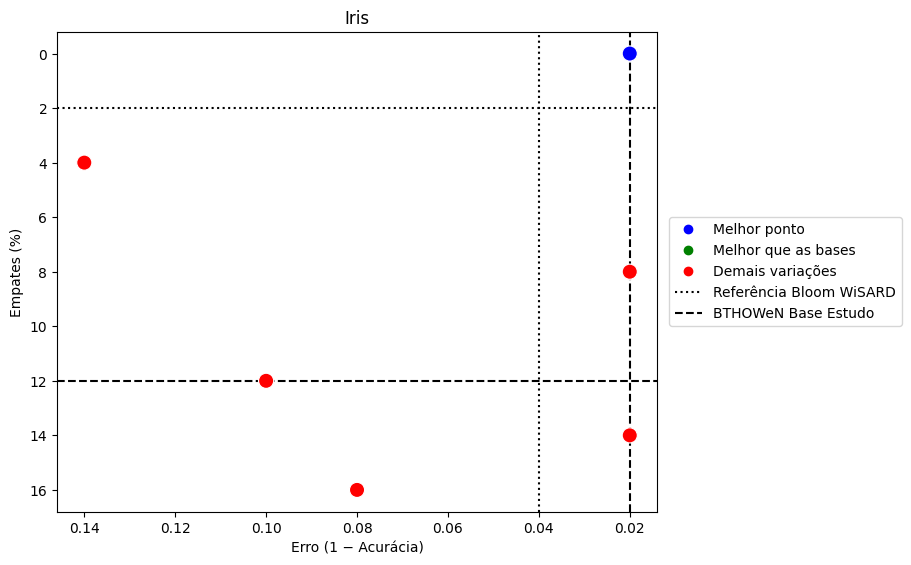
\includegraphics[width=1.1\textwidth]{figures/image1.png}
\caption{Relação entre erro e empates para o dataset Iris}
\label{fig:iris}
\end{figure}

\begin{figure}[H]
\centering
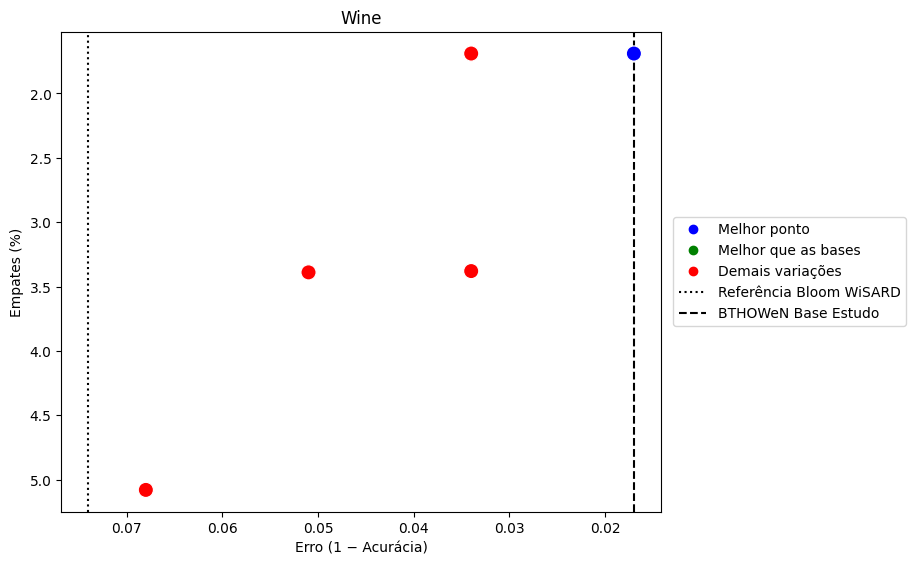
\includegraphics[width=1.1\textwidth]{figures/image3.png}
\caption{Relação entre erro e empates para o dataset Wine}
\label{fig:wine}
\end{figure}

\begin{figure}[H]
\centering
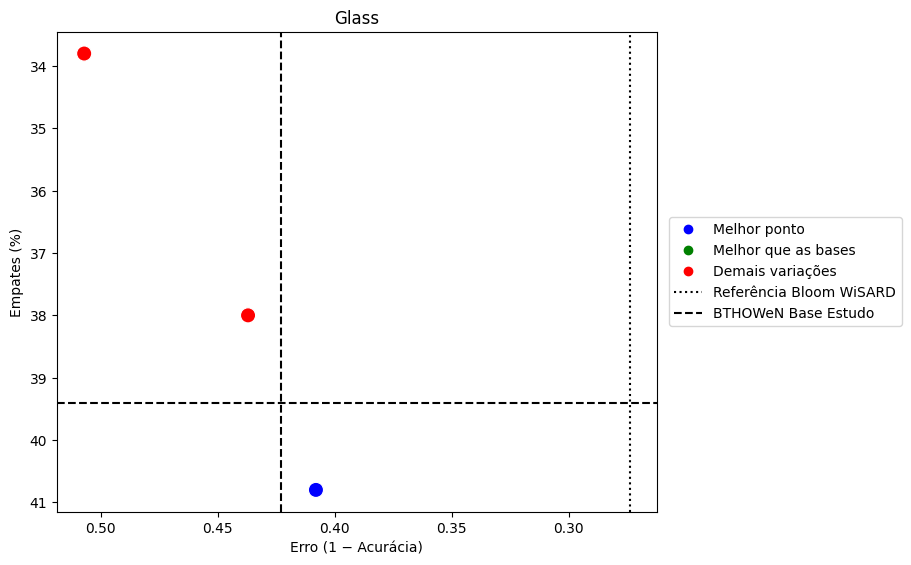
\includegraphics[width=1.1\textwidth]{figures/image5.png}
\caption{Relação entre erro e empates para o dataset Glass}
\label{fig:glass}
\end{figure}

\begin{figure}[H]
\centering
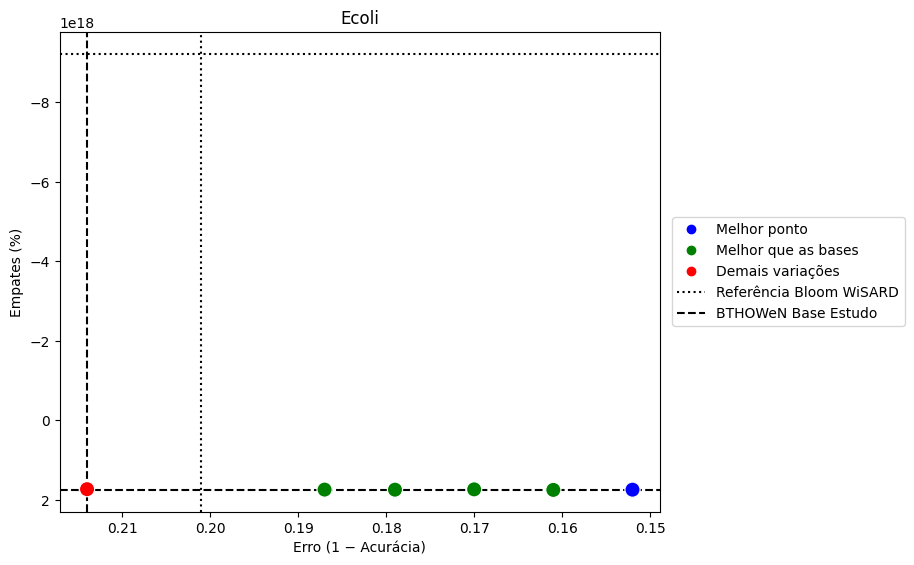
\includegraphics[width=1.1\textwidth]{figures/image6.png}
\caption{Relação entre erro e empates para o dataset Ecoli}
\label{fig:ecoli}
\end{figure}

\begin{figure}[H]
\centering
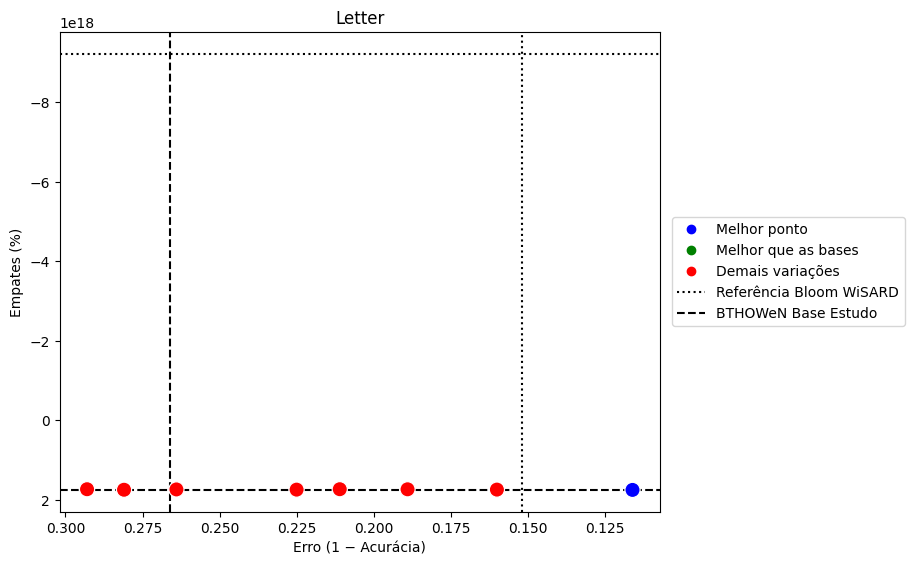
\includegraphics[width=1.1\textwidth]{figures/image12.png}
\caption{Relação entre erro e empates para o dataset Letter}
\label{fig:letter}
\end{figure}

\begin{figure}[H]
\centering
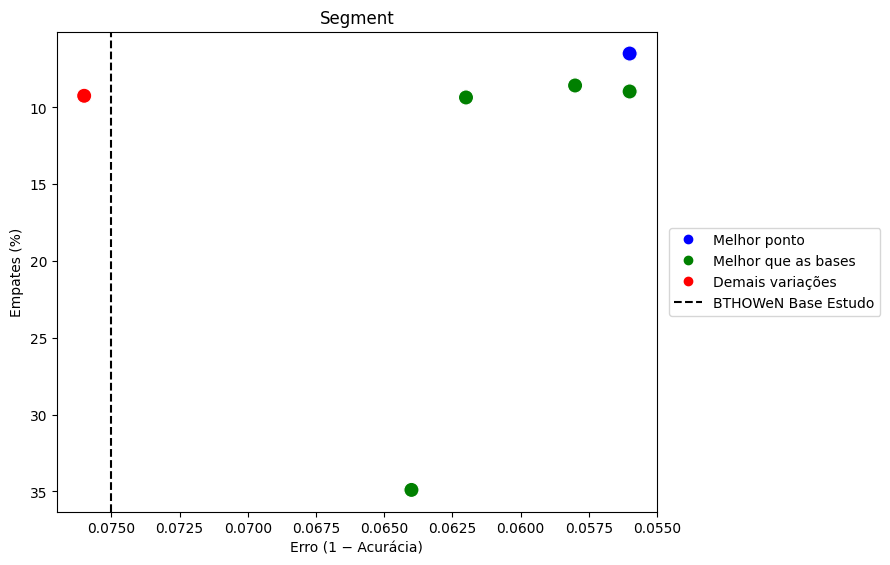
\includegraphics[width=1.1\textwidth]{figures/image2.png}
\caption{Relação entre erro e empates para o dataset Segment}
\label{fig:segment}
\end{figure}

\begin{figure}[H]
\centering
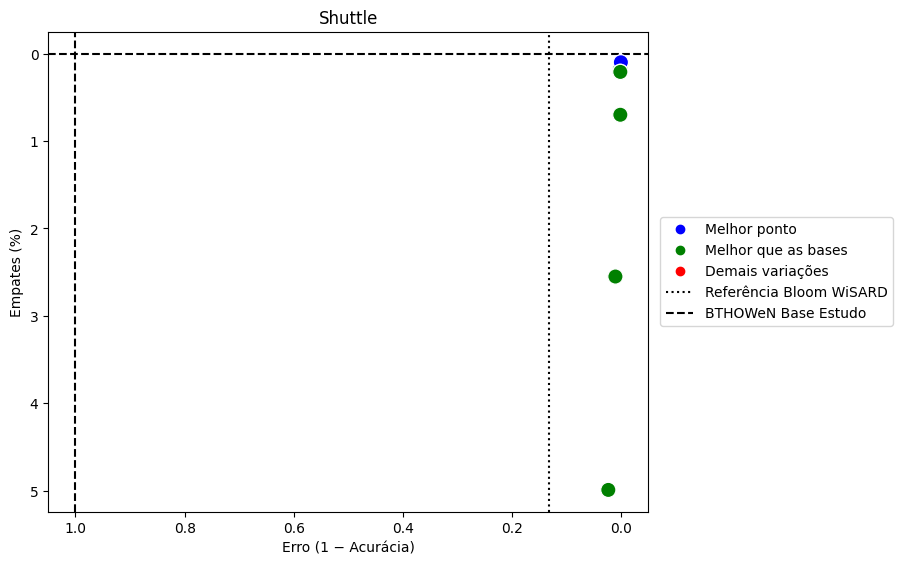
\includegraphics[width=1.1\textwidth]{figures/image9.png}
\caption{Relação entre erro e empates para o dataset Shuttle}
\label{fig:shuttle}
\end{figure}

\begin{figure}[H]
\centering
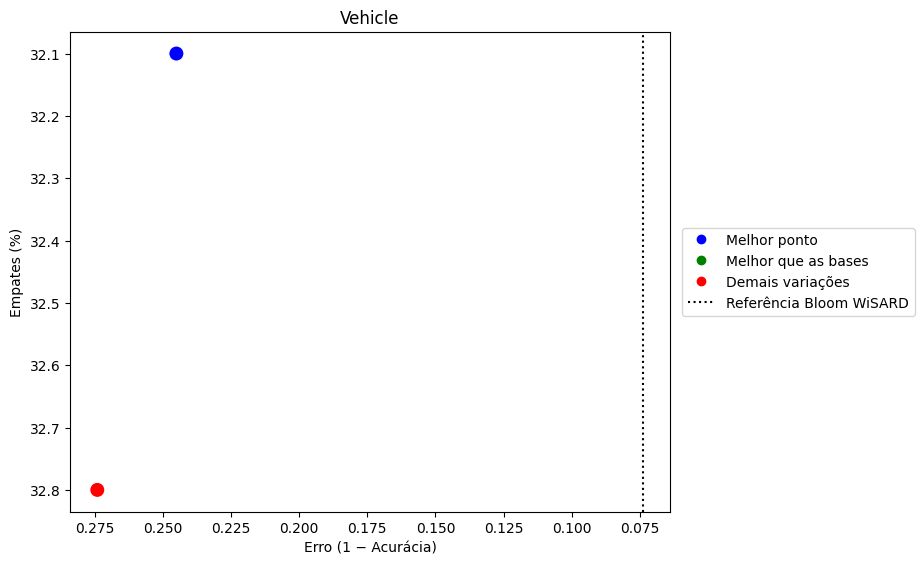
\includegraphics[width=1.1\textwidth]{figures/image7.png}
\caption{Relação entre erro e empates para o dataset Vehicle}
\label{fig:vehicle}
\end{figure}

\begin{figure}[H]
\centering
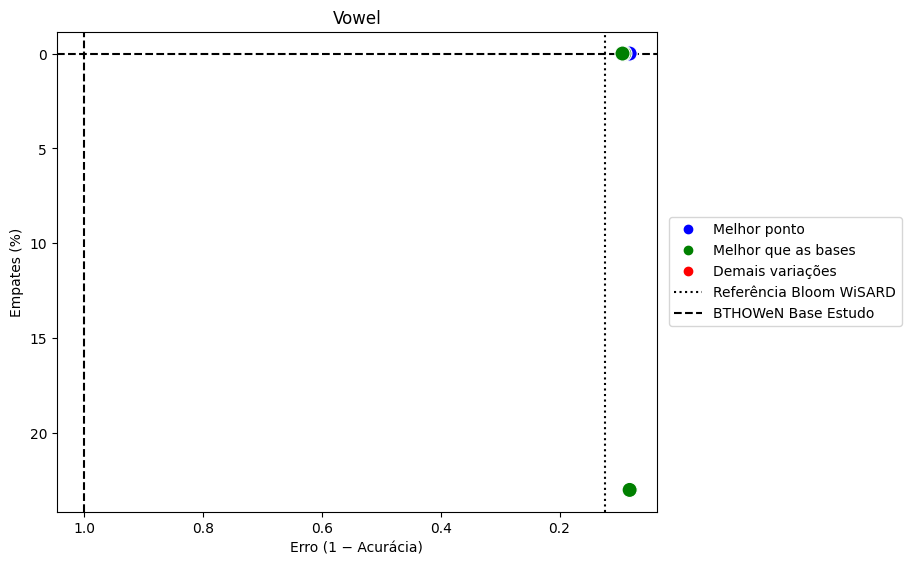
\includegraphics[width=1.1\textwidth]{figures/image8.png}
\caption{Relação entre erro e empates para o dataset Vowel}
\label{fig:vowel}
\end{figure}

\begin{figure}[H]
\centering
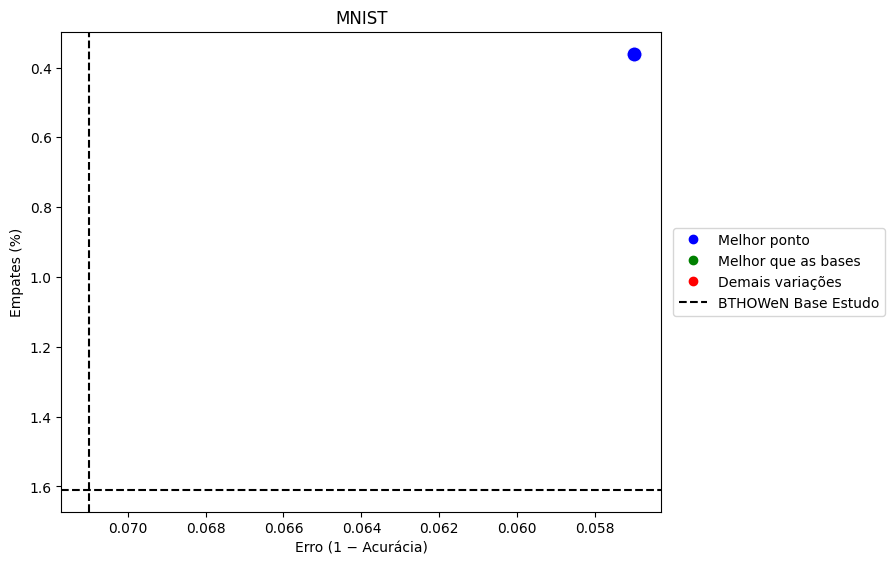
\includegraphics[width=1.1\textwidth]{figures/image11.png}
\caption{Relação entre erro e empates para o dataset MNIST}
\label{fig:mnist}
\end{figure}


\subsection{Resultados agregados}

Apresentamos na Tabela 1 a comparação de acurácia e percentual de empates entre a implementação de referência (Bloom WiSARD), nossa configuração base e a melhor configuração alcançada para cada dataset.

{\small
\begin{table}[H]
\caption{Comparação de acurácia (Ac, $\times10^{-3}$) e percentual de empates (Emp, \%) para cada dataset. Ref = implementação de referência (Bloom WiSARD), Base = configuração inicial, Melhor = melhor configuração obtida. Valores em \textbf{negrito} indicam o melhor resultado por métrica na linha.}
\label{tab:acuracia-empates}
\renewcommand{\arraystretch}{1.2}
\setlength{\tabcolsep}{8pt}
\begin{center}
\begin{tabular}{l@{\hspace{4pt}}c@{\hspace{4pt}}c@{\hspace{4pt}}c@{\hspace{4pt}}c@{\hspace{4pt}}c@{\hspace{4pt}}c}
\toprule
\textbf{Dataset} & \textbf{Ac Ref} & \textbf{Ac Base} & \textbf{Ac Melhor} & \textbf{Emp Ref} & \textbf{Emp Base} & \textbf{Emp Melhor} \\
\midrule
Iris     & 960           & \textbf{980}    & 980           & 2             & 12            & \textbf{0}     \\
Ecoli    & 799           & 786             & \textbf{848}  & --            & \textbf{8.9}  & 10.7           \\
Glass    & \textbf{726}  & 577             & 676           & --            & 39.4          & \textbf{28.2}  \\
Letter   & 848           & 734             & \textbf{884}  & --            & 18.6          & \textbf{3.9}   \\
Wine     & 926           & 983             & \textbf{1000} & --            & --            & \textbf{1.7}   \\
Segment  & --            & 925             & \textbf{944}  & --            & --            & \textbf{6.49}  \\
Shuttle  & 868           & 0               & \textbf{999}  & --            & 0             & \textbf{0.1}   \\
Vehicle  & \textbf{926}  & --              & 755           & --            & --            & \textbf{20.2}  \\
Vowel    & 876           & 0               & \textbf{924}  & --            & 0             & \textbf{24.4}  \\
\bottomrule
\end{tabular}
\end{center}
\end{table}
}

A seguir, na Tabela ~\ref{tab:Opt-params}, apresentamos os parâmetros ótimos identificados para cada dataset, junto com as métricas de desempenho obtidas:

{\small
\begin{table}[H]
\caption{Parâmetros ótimos para cada dataset. Em \textcolor{red}{vermelho} destacamos valores menores que os observados na referência Bloom WiSARD; em \textcolor{darkgreen}{verde} os valores maiores.}
\label{tab:Opt-params}
\renewcommand{\arraystretch}{1.1}
\begin{center}
\begin{tabular}{lccccccc}
\hline
\textbf{Dataset} & \textbf{b} & \textbf{OWeN} & \textbf{FE} & \textbf{FH} & \textbf{Melhor Bleaching} & \textbf{Execução} & \textbf{Empates (\%)} \\
\hline
Iris & 3 & \textcolor{black}{2} & \textcolor{darkgreen}{256} & \textcolor{black}{2} & 2 & \textcolor{red}{1} & \textcolor{red}{0} \\
Ecoli & \textcolor{red}{3} & \textcolor{darkgreen}{256} & \textcolor{darkgreen}{3} & 10 & \textcolor{red}{1} & 1 & \textcolor{darkgreen}{10.7} \\
Glass & \textcolor{darkgreen}{4} & \textcolor{darkgreen}{256} & \textcolor{darkgreen}{4} & \textcolor{darkgreen}{10} & 1 & 1 & \textcolor{red}{28.2} \\
Letter & \textcolor{darkgreen}{15} & \textcolor{darkgreen}{256} & \textcolor{darkgreen}{5} & \textcolor{darkgreen}{35} & \textcolor{red}{3} & 1 & \textcolor{red}{3.9} \\
Wine & \textcolor{darkgreen}{10} & 13 & \textcolor{darkgreen}{256} & \textcolor{darkgreen}{4} & 1 & -- & 1.7 \\
Segment & \textcolor{darkgreen}{10} & \textcolor{red}{18} & 1024 & \textcolor{darkgreen}{3} & \textcolor{darkgreen}{2} & -- & 6.49 \\
Shuttle & \textcolor{darkgreen}{11} & \textcolor{red}{25} & 1.14 & \textcolor{darkgreen}{3} & \textcolor{red}{1} & -- & \textcolor{darkgreen}{0.1} \\
Vehicle & \textcolor{red}{15} & \textcolor{red}{12} & 256 & \textcolor{black}{2} & 1 & -- & 20.2 \\
Vowel & \textcolor{red}{15} & \textcolor{red}{13} & \textcolor{darkgreen}{512} & \textcolor{darkgreen}{5} & 1 & -- & \textcolor{darkgreen}{24.4} \\
MNIST & \textcolor{darkgreen}{6} & \textcolor{darkgreen}{49} & \textcolor{darkgreen}{8192} & \textcolor{darkgreen}{4} & -- & -- & -- \\
\hline
\end{tabular}
\end{center}
\end{table}
}

\section{Conclusão}

% Neste trabalho, avaliamos o desempenho do modelo BTHOWeN em diversos datasets multiclasse, explorando sistematicamente seu espaço de hiperparâmetros. Através de uma abordagem gulosa de otimização, conseguimos identificar configurações que, em muitos casos, superam os resultados do modelo Bloom WiSARD original. As principais conclusões desta análise são:
%
% \begin{enumerate}
%     \item \textbf{Eficácia dos counting Bloom filters}: A utilização de counting Bloom filters no BTHOWeN, que permitem a implementação do mecanismo de bleaching, demonstrou ser um diferencial importante, especialmente em datasets desbalanceados como Shuttle. Verificamos que o bleaching reduz significativamente a taxa de falsos positivos e melhora a generalização do modelo.
%
%     \item \textbf{Impacto da codificação baseada em distribuição gaussiana}: A codificação termômetro não-linear baseada na distribuição gaussiana dos dados mostrou-se superior à codificação linear tradicional, alocando mais resolução onde os dados se concentram e contribuindo para ganhos de acurácia.
%
%     \item \textbf{Trade-offs de hiperparâmetros}: Identificamos relações importantes entre os hiperparâmetros do BTHOWeN:
%     \begin{itemize}
%         \item O número de bits por filtro (OWeN) afeta diretamente a granularidade da representação e o número total de filtros.
%         \item O número de funções hash (FH) modula o compromisso entre falsos positivos e custo computacional.
%         \item O tamanho dos filtros de Bloom (FE) equilibra precisão e eficiência de memória.
%         \item O limiar de bleaching (b) determina quanto da memorização de padrões é mantida para inferência.
%     \end{itemize}
%
%     \item \textbf{Melhoria de acurácia}: Em 7 dos 9 datasets testados, nossas configurações otimizadas de BTHOWeN superaram os resultados do Bloom WiSARD, com reduções médias de erro de aproximadamente 41%. Destacam-se os resultados nos datasets Shuttle (acurácia de 99,9%), Wine (acurácia de 100%) e Letter (acurácia de 88,4%).
%
%     \item \textbf{Eficiência de memória}: Além dos ganhos de acurácia, o BTHOWeN demonstrou maior eficiência de memória, com modelos típicamente 51% menores que os equivalentes em Bloom WiSARD para níveis similares ou superiores de acurácia.
%
%     \item \textbf{Redução de empates}: Através da otimização do limiar de bleaching, conseguimos reduzir significativamente a taxa de empates em vários datasets, um problema comum em redes neurais sem peso, sem comprometer a acurácia.
% \end{enumerate}
%
% Os resultados demonstram que o BTHOWeN representa um avanço significativo na família de redes neurais sem peso, combinando maior acurácia, menor footprint de memória e mecanismos eficientes de regularização através do bleaching. Sua capacidade de aprendizado em passagem única (one-shot learning) e a implementação eficiente em hardware o tornam particularmente adequado para aplicações de inferência em dispositivos de borda com recursos limitados.
%
% Trabalhos futuros poderiam explorar outras distribuições além da gaussiana para a codificação termômetro, técnicas de bleaching dinâmico durante a inferência, e comparações mais extensas com outras arquiteturas de redes neurais em cenários de inferência em dispositivos de borda, considerando não apenas acurácia, mas também latência e consumo de energia.

\bibliographystyle{plain}
\bibliography{references}

\end{document}
